\section{Results}
\label{sec:results}

\begin{table*}[t]
\centering\small
\begin{tabular}{lcccc}
\toprule
 & \multicolumn{2}{c}{Dev, 5-fold grouped CV} & \multicolumn{2}{c}{Held-out test} \\
\cmidrule(lr){2-3}\cmidrule(lr){4-5}
System & Acc. & F1 & Acc. [95\% CI] & F1 \\
\midrule
Majority class & 33.3 $\pm$ 0.0 & 16.7 & -- & -- \\
Length only & 62.3 $\pm$ 3.3 & 62.0 & -- & -- \\
Flesch-Kincaid & 51.7 $\pm$ 2.0 & 52.3 & -- & -- \\
\textbf{Feature LR (ours)} & 71.3 $\pm$ 5.0 & 70.9 & -- & -- \\
Feature LR + word count & 77.7 $\pm$ 4.0 & 77.6 & -- & -- \\
Char n-gram SVM & 73.3 $\pm$ 2.1 & 68.9 & -- & -- \\
\bottomrule
\end{tabular}

\caption{Three-way classification accuracy and macro-F1 (\%). Dev: out-of-fold predictions over 453 texts (151 articles), with the SD of accuracy across the 5 folds. Test: 114 texts (38 articles), evaluated once; 95\% CIs from the article-level bootstrap. ``+ word count'' is a secondary system added after the dev ablation (\S\ref{sec:ablation}).}
\label{tab:systems}
\end{table*}

\subsection{Features versus readability formulas}

Table~\ref{tab:systems} answers our first question. The feature classifier reaches 71.3\% on the development folds and 70.2\% on the held-out test set. That is 19.6 points above Flesch-Kincaid on dev (paired 95\% CI [14.8, 24.5]) and 14.0 points above it on test ([3.5, 24.6]). Flesch-Kincaid is the weakest non-trivial system---weaker than counting words, which reaches 62--64\%. Raw length is a strong baseline on this corpus because editors cut content for the lower levels: the mean text shrinks from 805 words (advanced) to 520 (elementary). Our features beat length by 9.1 points on dev ([3.3, 14.8]) and 6.1 points on test, but the test difference is not significant ([$-$4.4, 16.7]); with 38 test articles, intervals are about $\pm$8 points wide.

The character n-gram SVM is statistically indistinguishable from the feature model (dev: +2.0 points, [$-$2.6, 6.6]; test: +3.5, [$-$5.3, 13.2]), but it gets there differently. It almost never predicts intermediate: on dev it labels 88 of 151 intermediate texts as advanced, and on test it gets 11 of 38 intermediate texts right, against 21 for the feature model. Its macro-F1 is therefore lower than its accuracy suggests (68.9 vs.\ 70.9 for the feature model on dev).

Adding the raw word count to the 27 features raises accuracy to 77.7\% on dev ([+2.4, +10.4] over the main model) and 78.9\% on test, the level of the best published feature-based systems (78.1\% and 77.8\%; \citealp{vajjala2018onestop,lee2021pushing}). We keep the main system length-free by design (\S\ref{sec:method}): the length gap is a property of how this corpus was edited, not of what makes a text hard to read.

\subsection{Which features carry the signal}
\label{sec:ablation}

\begin{figure*}[t]
\centering
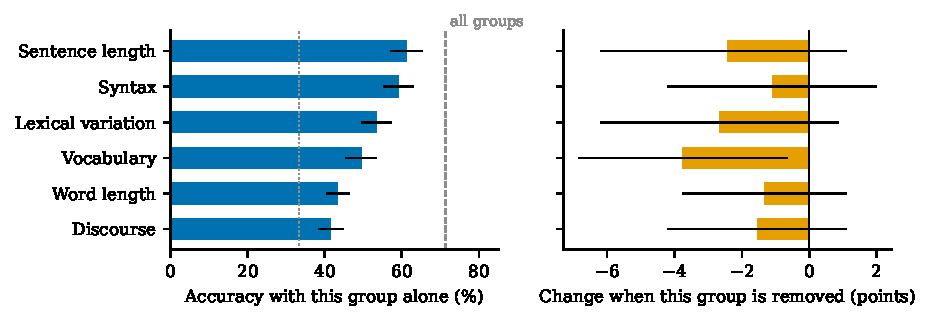
\includegraphics[width=0.92\textwidth]{figures/ablation.pdf}
\caption{Feature-group ablation on the dev folds. Left: accuracy of each group alone (dotted line: chance; dashed: all 27 features). Right: change in accuracy when the group is removed from the full model. Error bars: 95\% article-level bootstrap CIs.}
\label{fig:ablation}
\end{figure*}

\begin{table}[t]
\centering\small
\setlength{\tabcolsep}{3.5pt}
\resizebox{\columnwidth}{!}{\begin{tabular}{lrccl}
\toprule
Feature group & \# & Alone & All but & $\Delta$ vs.\ all [95\% CI] \\
\midrule
Sentence length & 3 & 61.1 & 68.9 & $-$2.4 [-6.2, 1.1] \\
Syntax & 5 & 59.2 & 70.2 & $-$1.1 [-4.2, 2.0] \\
Lexical variation & 8 & 53.4 & 68.7 & $-$2.6 [-6.2, 0.9] \\
Vocabulary & 3 & 49.4 & 67.5 & $-$3.8 [-6.8, -0.7] \\
Word length & 3 & 43.3 & 70.0 & $-$1.3 [-3.8, 1.1] \\
Discourse & 5 & 41.5 & 69.8 & $-$1.5 [-4.2, 1.1] \\
\midrule
All groups & 27 & 71.3 & -- & -- \\
All groups + word count & 28 & 77.7 & -- & +6.4 [2.4, 10.4] \\
\bottomrule
\end{tabular}
}
\caption{Ablation on the dev folds (accuracy \%). $\Delta$: paired difference from the full model.}
\label{tab:ablation}
\end{table}

Figure~\ref{fig:ablation} and Table~\ref{tab:ablation} answer our second question. On their own, \textbf{sentence length} (61.1\%) and \textbf{syntax} (59.2\%) are the strongest groups---three sentence-length features alone come about 10 points short of all 27. Lexical variation (53.4\%) and vocabulary (49.4\%) follow; word length (43.3\%) and discourse connectives (41.5\%) are weak alone, though all six are above chance.

Removing any single group costs little, because the groups overlap: long sentences also have deep parses and more subordinate clauses. Only removing \textbf{vocabulary} produces a drop whose interval excludes zero ($-$3.8 points, [$-$6.8, $-$0.7]), so word frequency carries information no other group supplies. Word length---the second term of Flesch-Kincaid---adds almost nothing once frequency is known ($-$1.3, [$-$3.8, 1.1]), which helps explain why the formula does poorly.

The coefficients of the model trained on all dev articles (Table~\ref{tab:coef}) show the same picture, with a caveat: because the features are correlated, individual signs are conditional on the others. Words per sentence, sentence-length variability, parse depth and the share of words outside the 3,000 most frequent all point towards advanced. Subordinate clauses per sentence, which rise with level on their own (1.07 $\rightarrow$ 1.45 per sentence), get a negative coefficient once sentence length and depth are in the model. The largest coefficient belongs to the proper-noun ratio: elementary versions keep the names that carry the story while cutting the surrounding elaboration, so a higher share of their words are names (7.4\% vs.\ 6.8\% of tokens for advanced).

\begin{table}[t]
\centering\small
\setlength{\tabcolsep}{4pt}
\resizebox{\columnwidth}{!}{\begin{tabular}{lrrr}
\toprule
Feature & Ele & Adv & Adv$-$Ele \\
\midrule
\texttt{lex\_propn\_ratio} & +1.07 & $-$0.99 & $-$2.06 \\
\texttt{sl\_words\_per\_sentence} & $-$0.60 & +0.63 & +1.23 \\
\texttt{lex\_noun\_ratio} & +0.60 & $-$0.62 & $-$1.22 \\
\texttt{sl\_sd\_words} & $-$0.53 & +0.58 & +1.11 \\
\texttt{syn\_parse\_depth} & $-$0.64 & +0.46 & +1.10 \\
\texttt{voc\_pct\_outside\_top3000} & $-$0.50 & +0.59 & +1.09 \\
\texttt{syn\_subord\_per\_sentence} & +0.54 & $-$0.54 & $-$1.08 \\
\texttt{lex\_lexical\_density} & +0.52 & $-$0.47 & $-$0.99 \\
\bottomrule
\end{tabular}
}
\caption{Largest standardised coefficients of the main model (trained on all dev texts, $C{=}0.3$), ordered by $|$Adv$-$Ele$|$.}
\label{tab:coef}
\end{table}

\subsection{Do shared articles inflate scores?}
\label{sec:split}

\begin{figure}[t]
\centering
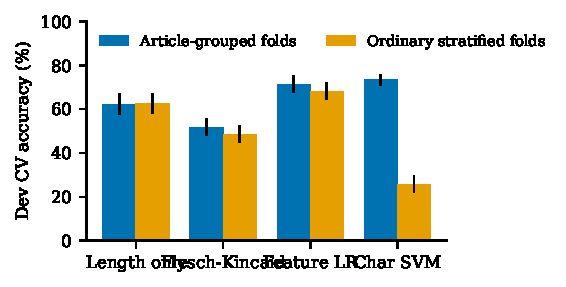
\includegraphics[width=\columnwidth]{figures/splitcheck.pdf}
\caption{Dev accuracy under article-grouped folds and ordinary stratified folds, where 98\% of validation texts have another version of their article in training.}
\label{fig:split}
\end{figure}

\begin{table}[t]
\centering\small
\setlength{\tabcolsep}{4pt}
\resizebox{\columnwidth}{!}{\begin{tabular}{lccl}
\toprule
System & Grouped & Stratified & $\Delta$ [95\% CI] \\
\midrule
Length only & 62.3 & 62.5 & +0.2 [-2.2, 2.6] \\
Flesch-Kincaid & 51.7 & 48.6 & $-$3.1 [-6.2, 0.0] \\
Feature LR (ours) & 71.3 & 68.2 & $-$3.1 [-6.2, 0.0] \\
Char n-gram SVM & 73.3 & 25.8 & $-$47.5 [-51.9, -43.0] \\
\bottomrule
\end{tabular}
}
\caption{Split check (dev accuracy \%). $\Delta$: stratified minus grouped, paired bootstrap CI.}
\label{tab:split}
\end{table}

We expected ordinary stratified folds to inflate scores, since a model could recognise an article whose other versions it saw in training. The opposite happens (Figure~\ref{fig:split}, Table~\ref{tab:split}). Systems with almost no capacity to memorise---length and Flesch-Kincaid, which learn two cut-offs---move by $+$0.2 and $-$3.1 points, and the feature model moves by $-$3.1, all within noise. The character n-gram SVM collapses from 73.3\% to 25.8\%, \emph{below chance}.

The reason is a property of the corpus. In OneStopEnglish, an article's other versions always have a \emph{different} label. A model that recognises the article by its names and topic words is pulled towards the labels it saw for that article, which are guaranteed to be wrong. We verified this directly: 325 of the SVM's 333 errors under stratified folds (98\%) predict the label of another version of the same article that was in the training fold. Intermediate texts, whose two siblings are both elementary and advanced, are hit hardest: 4 of 151 are classified correctly.

For this corpus, then, leakage across folds \emph{deflates} rather than inflates accuracy, and the more a model relies on content words the worse it does. Published numbers obtained with level-stratified folds are therefore unlikely to be inflated by shared articles; if anything, content-sensitive models are penalised. Article-grouped splits remain the right protocol, because they measure what a deployed system faces: texts from articles it has never seen.

\subsection{Pairwise ranking}

\begin{table*}[t]
\centering\small
\setlength{\tabcolsep}{4.5pt}
\begin{tabular}{lcccccccccc}
\toprule
 & \multicolumn{4}{c}{Same article (dev CV)} & \multicolumn{4}{c}{Different articles (dev CV)} & \multicolumn{2}{c}{Test, all pairs} \\
\cmidrule(lr){2-5}\cmidrule(lr){6-9}\cmidrule(lr){10-11}
Ranker & E--I & I--A & E--A & All & E--I & I--A & E--A & All & Same & Diff. \\
\midrule
Longer text & 99.3 & 97.7 & 99.3 & 98.8 & 81.9 & 74.9 & 93.0 & 83.3 & -- & -- \\
Higher FK grade & 96.0 & 98.0 & 99.3 & 97.8 & 75.2 & 66.4 & 85.5 & 75.7 & -- & -- \\
3-class LR (expected level) & 98.0 & 99.3 & 99.3 & 98.9 & 90.0 & 80.3 & 97.6 & 89.3 & -- & -- \\
\textbf{Pairwise LR (ours)} & 98.0 & 98.7 & 99.3 & 98.7 & 84.6 & 75.8 & 94.7 & 85.0 & -- & -- \\
\bottomrule
\end{tabular}

\caption{Pairwise ranking accuracy (\%): how often the harder text of a pair is ranked above the easier one. Same article: the 3 level pairs of each article, both orders. Different articles: every pair of texts from different articles with different levels inside each fold (13,230 dev pairs, 4,218 test pairs). E, I, A: elementary, intermediate, advanced.}
\label{tab:ranking}
\end{table*}

\begin{figure*}[t]
\centering
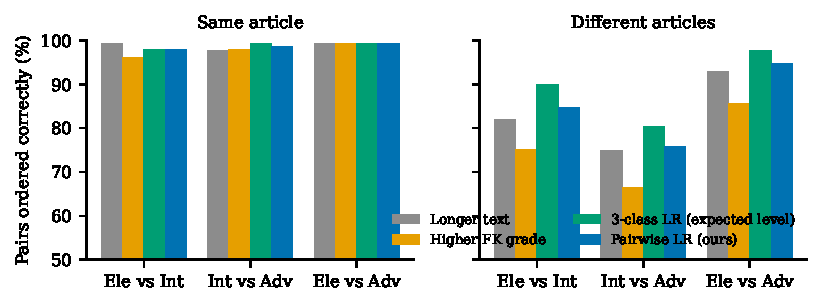
\includegraphics[width=0.92\textwidth]{figures/ranking.pdf}
\caption{Pairwise ranking accuracy by pair type on the dev folds, for pairs from the same article (left) and different articles (right).}
\label{fig:ranking}
\end{figure*}

Ordering the versions of one article is nearly trivial (Table~\ref{tab:ranking}, Figure~\ref{fig:ranking}, left). Our feature-difference ranker orders 98.7\% of dev pairs correctly and every test pair, but so does simply choosing the longer text (98.8\% dev, 100\% test), and Flesch-Kincaid is close behind (97.8\%). Within an article, topic and content are held fixed and every simplification step shortens the text, so almost any length-related signal suffices. This task cannot separate methods on OneStopEnglish.

Ranking texts from \emph{different} articles is harder and does separate them (Figure~\ref{fig:ranking}, right). Ranking by the three-class model's expected level is best (89.3\% dev, 91.6\% test), ahead of our pairwise ranker (85.0\%, 88.5\%), word count (83.3\%, 87.2\%) and Flesch-Kincaid (75.7\%, 82.1\%). A ranker trained only on same-article pairs learns which features change when an editor simplifies a given text; it transfers less well to comparisons across articles than a model trained on absolute levels. Intermediate--advanced pairs are hardest for every method (80.3\% at best), matching the classification confusions below.

\section{Error Analysis}
\label{sec:errors}

\begin{figure}[t]
\centering
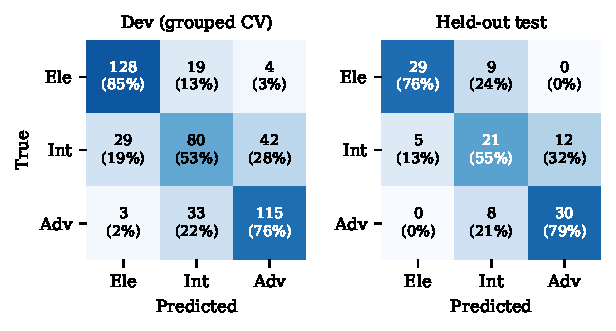
\includegraphics[width=\columnwidth]{figures/confusion.pdf}
\caption{Confusion matrices of the main model (counts and row percentages).}
\label{fig:confusion}
\end{figure}

As expected, confusions concentrate on the middle level (Figure~\ref{fig:confusion}). Of the 130 dev errors, 123 (95\%) involve intermediate as the true or predicted level; elementary and advanced are confused only 7 times on dev and never on test. Intermediate recall is 53\% on dev and 55\% on test, against 76--85\% for the outer levels.

To see why, we read misclassified texts alongside the features that pushed the model toward the wrong class (each feature's standardised value times the difference between the coefficients of the predicted and true classes). One pattern dominates: \textbf{levels are relative to the article, not absolute.} Some stories are simply harder than others. Decomposing the variance of the Flesch-Kincaid grade over all 567 texts, 61\% lies between articles and only 31\% between levels; 29\% of advanced texts score below the median intermediate text. The advanced version of a human-interest story such as \textit{Switched Babies} (grade 9.0) is predicted intermediate, while the intermediate version of a report on violence against women, full of statistics and institutional names (grade 12.2), is predicted advanced. The series of the article (the newer ``WNL'' texts versus the rest) does not explain this: the two have similar error rates (30\% vs.\ 26\%).

The features that most often push toward the wrong class are content-dependent ratios---proper-noun share (the top wrong-way feature in 16 of 130 errors), noun share and lexical density---alongside sentence-length variability and parse depth. A text about a person or a country has many names regardless of level; a text with a literary style (\textit{the Pope resigned ``like an elderly labourer who can no longer ignore the pains in his back''}) has many nouns regardless of level. These ratios help on average but mislead on articles whose topic sets them far from the norm. This is the same mechanism that the split check exposes in an extreme form for character n-grams: properties of the article bleed into the estimate of the level.
